% Scene C of "Render a ping without Gazebo" (render-a-ping.md), from gz_sonar/examples/render_ping.cc:
% imaging sonar as in scene B (2 m up, pitched down 15 deg, 120 x 20 deg, 10 m window) over a seabed rising 10 deg to
% starboard (-y), through the point under the sonar.
% (a) looking forward along the sonar's heading: port left, starboard right. True scale, 1 unit = 1 m.
% (b) plan view, forward to the right, port up: where the seabed first enters the beam (the lower beam edge, 10 deg
%     below the axis, meeting the seabed), for the flat seabed of scene B (dashed) and the slope of scene C (solid),
%     clipped to the fan and the 10 m window.
% Build: pdflatex render_ping_C.tex, then pdftocairo to ../images/render_ping_C.{png,svg}
\documentclass[tikz,border=6pt]{standalone}
\usetikzlibrary{arrows.meta,calc}
\renewcommand{\familydefault}{\sfdefault}
\tikzset{
  lbl/.style={font=\sffamily\small},
  beam/.style={fill=black!7,draw=black,thin},
  dim/.style={thin,{Latex[length=1.6mm]}-{Latex[length=1.6mm]}},
  lead/.style={thin,black!70},
  axis/.style={thin,dashed},
  shadow/.style={fill=black!30,draw=none},
}
% seabed line from x0 to x1 at height z (drawing units), slab of dots below
\newcommand{\seabed}[3]{
  \draw[thick] (#1,#3) -- (#2,#3);
  \foreach \r [count=\i] in {0.12,0.3} {
    \pgfmathsetmacro{\o}{mod(\i,2)*0.12}
    \pgfmathsetmacro{\n}{int((#2-#1-0.3)/0.24)}
    \foreach \k in {0,...,\n} \fill ({#1+0.12+\k*0.24+\o},{#3-\r}) circle (0.4pt);
  }
}
% sonar head at #1, pitched down #2 degrees
\newcommand{\head}[2]{
  \begin{scope}[shift={#1},rotate=-#2]
    \draw[fill=black!15] (-0.5,-0.13) rectangle (0,0.13);
    \fill (0,0) circle (1.4pt);
  \end{scope}
}
\begin{document}
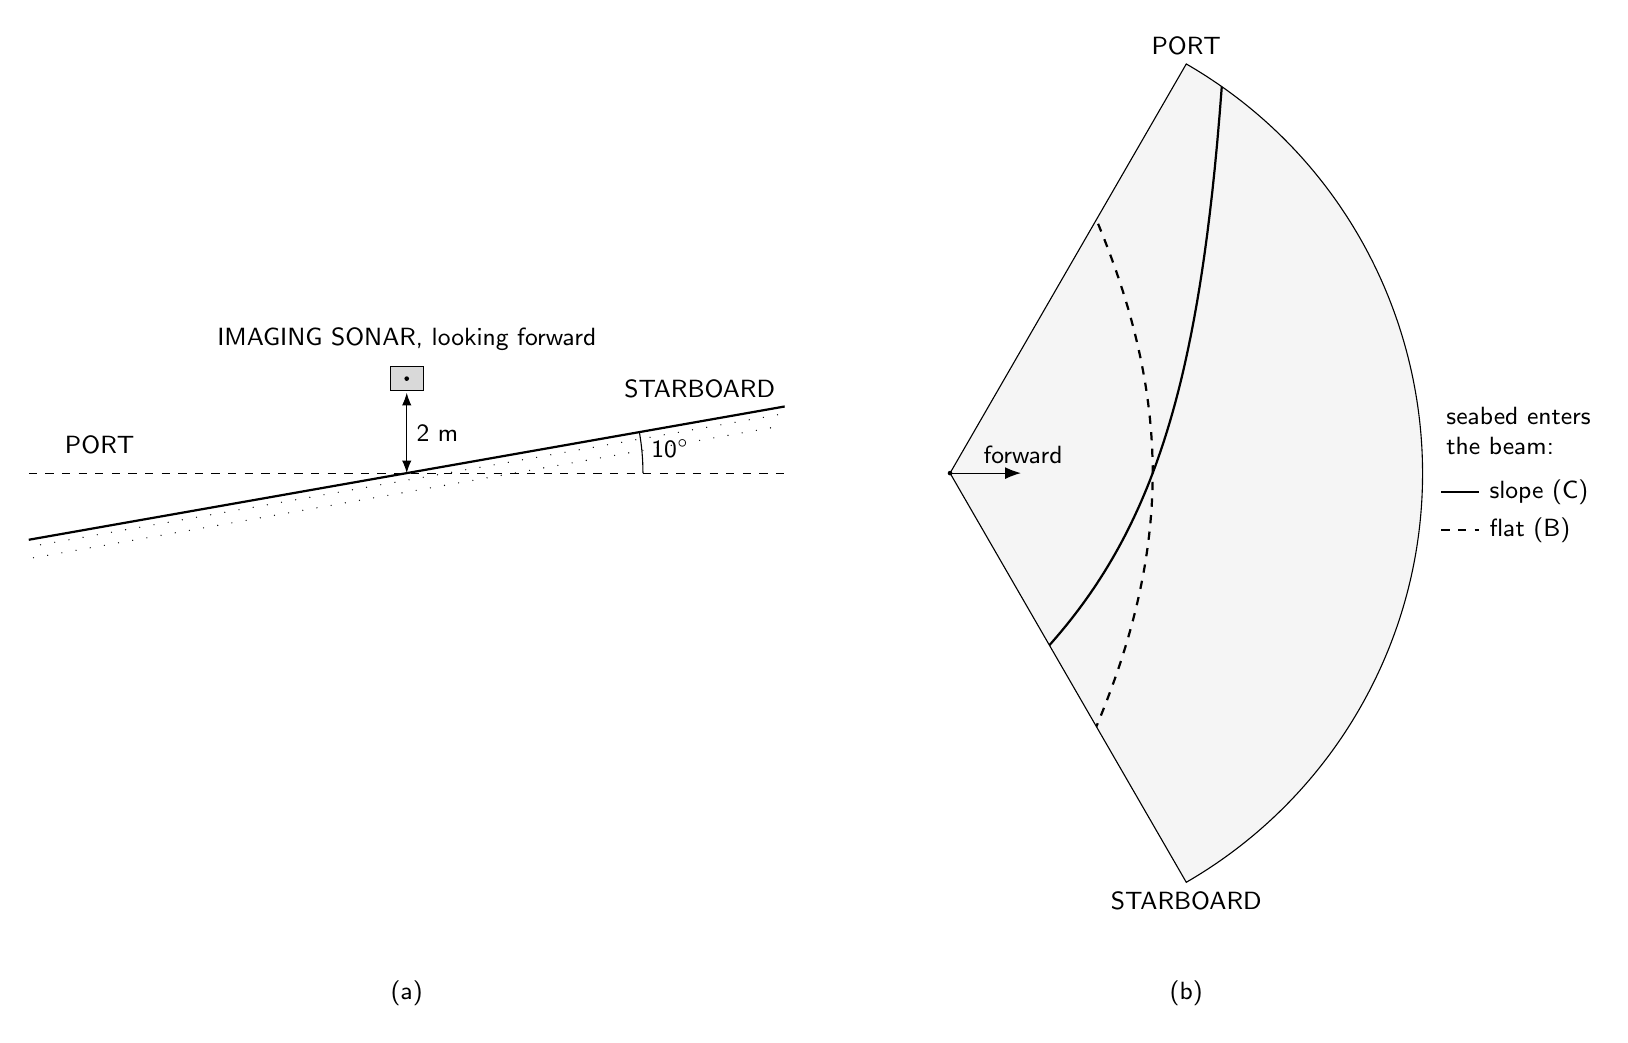
\begin{tikzpicture}[scale=0.6]
  % ---------------- (a) looking forward
  \begin{scope}
    \draw[thick] (-8,{-8*tan(10)}) -- (8,{8*tan(10)});
    \foreach \r [count=\i] in {0.15,0.4} {
      \pgfmathsetmacro{\o}{mod(\i,2)*0.15}
      \foreach \u in {-7.9,-7.6,...,7.8} \fill ({\u+\o},{(\u+\o)*tan(10)-\r}) circle (0.4pt);
    }
    \draw[axis] (-8,0) -- (8,0);
    \draw (5,0) arc (0:10:5) node[lbl,anchor=west,pos=0.6] {10$^\circ$};
    \draw[fill=black!15] (-0.35,1.75) rectangle (0.35,2.25);
    \fill (0,2) circle (1.4pt);
    \draw[dim] (0,1.7) -- (0,0) node[lbl,midway,right] {2 m};
    \node[lbl,anchor=south] at (-6.5,0.2) {PORT};
    \node[lbl,anchor=south] at (6.2,1.4) {STARBOARD};
    \node[lbl,anchor=south] at (0,2.4) {IMAGING SONAR, looking forward};
    \node[lbl] at (0,-11) {(a)};
  \end{scope}
  % ---------------- (b) plan view
  \begin{scope}[shift={(11.5,0)}]
    \draw[beam,fill=black!4] (0,0) -- (60:10) arc (60:-60:10) -- cycle;
    \begin{scope}
      \clip (0,0) -- (60:10) arc (60:-60:10) -- cycle;
      % flat seabed (scene B): t = -2 / wz
      \draw[thick,dashed] plot[domain=-60:60,samples=61] (
        {-2/(-sin(15)*cos(10)*cos(\x)+cos(15)*sin(-10))*(cos(15)*cos(10)*cos(\x)+sin(15)*sin(-10))},
        {-2/(-sin(15)*cos(10)*cos(\x)+cos(15)*sin(-10))*cos(10)*sin(\x)});
      % seabed rising to starboard (scene C): t = -2 cos10 / (sin10 wy + cos10 wz)
      \draw[thick] plot[domain=-60:60,samples=61] (
        {-2*cos(10)/(sin(10)*cos(10)*sin(\x)+cos(10)*(-sin(15)*cos(10)*cos(\x)+cos(15)*sin(-10)))*(cos(15)*cos(10)*cos(\x)+sin(15)*sin(-10))},
        {-2*cos(10)/(sin(10)*cos(10)*sin(\x)+cos(10)*(-sin(15)*cos(10)*cos(\x)+cos(15)*sin(-10)))*cos(10)*sin(\x)});
    \end{scope}
    \fill (0,0) circle (1.4pt);
    \draw[-{Latex[length=2mm]}] (0,0) -- (1.5,0) node[lbl,anchor=south] {\,forward};
    \node[lbl,anchor=south] at (60:10) {PORT};
    \node[lbl,anchor=north] at (-60:10) {STARBOARD};
    \node[lbl,anchor=west,align=left] at (10.3,0.9) {seabed enters\\the beam:};
    \draw[thick] (10.4,-0.4) -- ++(0.8,0) node[lbl,anchor=west] {slope (C)};
    \draw[thick,dashed] (10.4,-1.2) -- ++(0.8,0) node[lbl,anchor=west] {flat (B)};
    \node[lbl] at (5,-11) {(b)};
  \end{scope}
\end{tikzpicture}
\end{document}
